\section{Elements of continuum mechanics}
\label{sec:principles:continuumMechanics}

This section recapitulates the basic notions from continuum mechanics
and the associated shorthand notations that will be used throughout
the text. We define the coordinate system, described by the axes
$\unitV{i}~,~i=1 \ldots 3$. Throughout the text \emph{Einstein
  notation} is used, meaning that a repeated index $i$ implies a
summation:
\begin{align*}
  a_i b_i \hat = \sum_i a_i b_i 
\end{align*}

\subsection{State variables and tensors}
\label{subsec:principles:tensors}

We only consider \emph{intensive} state variables, \ie that define the
flow locally. Strictly speaking tensors are intensive state variables
which are frame independent (\ie only a component transformation
following the change of coordinate system is required to know them in
any frame). We rank tensors following order, \ie the number of indices
required to identify a component. The term tensors will be used
loosely however, to include frame-dependent quantities.

\subsubsection{Scalar quantities} 

\emph{Scalars} or \emph{zero-th order tensors} are denoted throughout
the text in normal face. Common scalar quantities in this course are
given in table \ref{tab:scalars}:
\begin{table}[H]
  \centering{
    \begin{tabular}{lccr}
      quantity & symbol & & units \\
      \hline
      density & \dens &  & $[kg/m^3]$ \\
      specific volume & $\sVol$ & $1/\dens$ & $[m^3/kg]$ \\
      pressure & \pres & &$[Pa]$ \\
      temperature & \temp & &$[K]$ \\
      internal energy & \ener && $[J/kg]$ \\
      enthalpy & \enth & & $[J/kg]$ \\
      entropy & \entr & & $[J/kg K]$ \\
      \hline
      total enthalpy & \tEnth & & $[J/kg]$ \\
      total internal energy & \tEner & & $[J/kg]$\\
    \end{tabular}}
  \caption{Common scalar quantities in fluid mechanics}
  \label{tab:scalars}
\end{table}
\noindent
Both \tEnth~ and \tEner~ are frame dependent scalars and therefore not
strictly speaking tensors.
  
\subsubsection{Vectors} 

\emph{Vectors} or \emph{first order tensors} $\mathbf a$ are noted in
bold face. Common vectors used in this course are listed in table
\ref{tab:vectors}:
\begin{table}[H]
  \centering{
    \begin{tabular}{lcc}
      Quantity & symbol & units \\
      \hline
      gravitational acceleration & \gravV & $[m/s^2]$ \\
      absolute flow velocity     & \aVelV & $[m/s]$   \\
      absolute frame velocity    & \fVelV & $[m/s]$   \\
      frame rotation vector      & \rotV  & $[rad/s]$ \\
      \hline
      position$^\ast$             & \xyzV  & $[m]$ \\
      relative flow velocity$^\ast$ & \rVelV & $[m/s]$\\
    \end{tabular}
  }
  \caption{Common vector quantities}
  \label{tab:vectors}
\end{table}
In general, the components of a vector will be noted following the
convention $\mathbf a = a_i \unitV{i}$, with the exception of the
position vector where $\xyzV = x_i \unitV{i}$, since $\xyz$ will be
reserved for the norm $||\xyzV||$. Both position and relative velocity
are not actually vectors since they are frame dependent.

\subsubsection{Inner product of two vectors}
  
The \emph{inner} or \emph{dot} product of two vectors $\mathbf a$ and
$\mathbf b$ results in a scalar:
\begin{align*}
  \mathbf a \cdot \mathbf b 
  &= \left(a_i \unitV{i}\right) \cdot \left(b_j \unitV{j}\right) 
  = (a_i b_j) ~\unitV{i} \cdot \unitV{j} 
  = (a_i b_j) ~\delta_{ij} 
  = a_i b_i
\end{align*}
with $\delta_{ij}$ the \emph{Kronecker symbol}, defined as follows:
\begin{itemize}
\item $\delta_{ij} = 1$ if $i=j$;
\item $\delta_{ij}=0$ if $i\neq j$.
\end{itemize}

\subsubsection{Vector product}

The vector product $\mathbf a \times \mathbf b$ can be compactly noted. We start by decomposing $\mathbf a$ and $\mathbf b$ following the unit vectors. We find that 
\begin{align*}
    \mathbf a \times \mathbf b &= a_i \unitV{i} \times b_j \unitV{j} \\
        &= a_i b_j \left(\left(\unitV{i} \times \unitV{j}\right) \cdot \unitV{k}\right) \unitV{k} \\
        &= a_i b_j \epsilon_{ijk} \unitV{k}
\end{align*}
with $\epsilon_{ijk}=(\unitV{i} \times \unitV{j})\cdot \unitV{k}$ the \emph{Levi-Civit{\`a}} symbol, with the following values
\begin{itemize}
\item $\epsilon_{ijk} = 1$ if $(\unitV{i},\unitV{j},\unitV{k})$ form a
  right-handed system of axes;
\item $\epsilon_{ijk} = -1$ if $(\unitV{i},\unitV{j},\unitV{k})$ form a
  left-handed system of axes;
\item $\epsilon_{ijk} = 0$ otherwise, \ie if any of the indices are repeated.
\end{itemize}
Then one can easily prove the following identity 
\begin{align*}
    \epsilon_{ijk} \epsilon_{lmk} = \delta_{il} \delta_{jm} - \delta_{im} \delta_{jl}
\end{align*}

\subsubsection{Outer product of two vectors}

The \emph{outer} or \emph{dyadic} product $\mathbf a \mathbf b$ of two
vectors $\mathbf a$ and $\mathbf b$ results in a matrix-like structure
with two indices
\begin{align*}
  (\mathbf a \mathbf b)_{ij} = a_i b_j
\end{align*}
or equivalently
\begin{align*} 
  \mathbf a \mathbf b = 
  \begin{bmatrix} 
    a_1 b_1 & a_1 b_2 & a_1 b_3 \\
    a_2 b_1 & a_2 b_2 & a_2 b_3 \\
    a_3 b_1 & a_3 b_2 & a_3 b_3 \\
  \end{bmatrix}
\end{align*}
One can easily check that the resulting matrix has rank 1, and that
conversely any matrix of rank 1 can be decomposed as a dyadic
product. Sometimes we will note the outer product rather as $\mathbf a
\otimes \mathbf b$ for clarity.

A convenient notation of the dyadic product is to express it as a sum
of the outer product of the unit vectors
\begin{align*}
  \mathbf a \mathbf b = a_i b_j \unitV{i} \unitV{j} = 
  a_1 b_1 
  \begin{bmatrix} 1 & 0 & 0 \\ 0 & 0 & 0 \\ 0 & 0 & 0 \end{bmatrix} +
  a_1 b_2 
  \begin{bmatrix} 0 & 1 & 0 \\ 0 & 0 & 0 \\ 0 & 0 & 0 \end{bmatrix} +
  \ldots +
  a_3 b_3
  \begin{bmatrix} 0 & 0 & 0 \\ 0 & 0 & 0 \\ 0 & 0 & 1 \end{bmatrix} 
\end{align*}
The outer product can be pre- or post-multiplied by vectors 
\begin{align*}
  \mathbf a \cdot \mathbf b \mathbf c = (\mathbf a \cdot \mathbf b) \mathbf c \\
  \mathbf a \mathbf b \cdot \mathbf c = \mathbf a (\mathbf b \cdot \mathbf c) \\
\end{align*}
In this instance, we can see that the notation in unit vectors is
rather useful, \eg for the premultiplication
\begin{align*}
  \mathbf a \cdot \left(\mathbf b \mathbf c\right) &= a_i \unitV{i} \cdot \left(b_j c_k ~\unitV{j} \unitV{k} \right) \\
  &= a_i b_j c_k ~\left(\unitV{i} \cdot  \unitV{j}\right) \unitV{k} \\
  &= a_i b_j c_k ~ \delta_{ij} ~\unitV{k} \\
  %%&= a_i b_i ~ c_k ~ \unitV{k} \\
  &= \left(\mathbf a \cdot \mathbf b\right) \mathbf c
\end{align*}
% An example of a outer product is the momentum flux tensor $\dens
% \aVelV \aVelV$; the flux of momentum across a surface $S$ with normal
% $\nrmV$ is
% \begin{align*}
%   \int_S \dens \aVelV \aVelV \cdot \nrmV dS = \int_S \aVelV \left(\dens \aVelV \cdot \nrmV\right) dS = \int_S d \mFlow \aVelV
% \end{align*}

\subsubsection{Dyadics or second order tensors}

Generalizing from the outer product, we can define more general
two-dimensional structures called \emph{dyadics} or \emph{second order
  tensors}. Dyadics are not restricted to rank-1 matrices, and will
typically noted in bold greek letters:
\begin{align*}
  \boldsymbol \gamma = \gamma_{ij} \unitV{i} \unitV{j}
\end{align*}
The pre- or postmultiplication then results in 
\begin{align*}
  \mathbf a \cdot \boldsymbol \gamma = a_i \gamma_{ij} \unitV{j} \\
  \boldsymbol \gamma \cdot \mathbf b = \gamma_{ij} b_j \unitV{i} \\
\end{align*}
\begin{figure}[!h]
  \centering
  \includegraphics[width=0.3\textwidth]{principles/stress.png}
  \caption{Stress tensor definition (Wikimedia commons)}
  \label{fig:stress}
\end{figure}
An important example of a dyadic is the stress tensor $\stressT$ in
the fluid, generated by the interaction with surrounding fluid
particles, through \emph{pressure} $p$, generating a purely normal
contribution, and \emph{shear stress} $\shearStressT$, generating
(mainly) a tangential contribution:
\begin{align*} 
  \stressT = \left(- p \delta_{ij} + \shearStress_{ij}\right)
  \unitV{i} \unitV{j} = -p \identityT + \shearStressT
\end{align*}
with \identityT~ the identity tensor.  The force on any surface
exerted by stress is found by the projection on its normal $\nrmV$, as
shown in figure \ref{fig:stress}
\begin{align*}
  \mathbf T^{\nrmV} = \stressT \cdot \nrmV
\end{align*}

\subsubsection{Inner product of two dyads}

As for vectors, we can define an inner product for two dyads by summing the products of all corresponding entries:
\begin{align*}
        \boldsymbol \kappa : \boldsymbol \lambda = \kappa_{ij} \lambda_{ij}
\end{align*}

\subsection{Gradient operators}
\label{subsec:principles:gradientOperators}

In order to derive complex gradient operator expressions, the nabla
$\nabla$ operator can be formally noted in the same way as a vector
\begin{align*}
  \grad \hat =  \dd{}{x_i} \unitV{i}
\end{align*}
to combine it with the tensor notations in the previous
subsection. 

\subsubsection{Gradient of a scalar} 

It is formally noted as the multiplication of the gradient vector and
the scalar a:
\begin{align*}
  \grad a =  \dd{a}{x_i} ~\unitV{i}
\end{align*}
As an example, the heat flux vector is modeled by \emph{Fourier's}
law, stating that heat flows from high to low temperature, with fluxes
proportional and opposite to the temperature gradient
\begin{align*}
  \heatFluxV = - \conduct \grad T
\end{align*}
with \conduct~ the \emph{conductivity}.

\subsubsection{Divergence of a vector} 

The divergence of a vector is a scalar, which can formally be noted as the inner product of the nabla vector $\nabla$ and the vector $\mathbf a$
\begin{align*}
  \dive \mathbf a 
  = \left(\dd{}{x_i} \unitV{i}\right) \cdot (\mathbf a_j \unitV{j}) 
  = \dd{a_j}{x_i} \left(\unitV{i} \cdot \unitV{j}\right) = \dd{a_j}{x_i}~\delta_{ij} 
  = \dd{a_i}{x_i}
\end{align*}

\subsubsection{Gradient of a vector}

The gradient of a vector $\mathbf a$ is a dyad, which can be formally noted as the outer product of
the gradient vector and $\mathbf a$:
\begin{align*}
  \grad \mathbf a 
  = \left(\dd{}{x_i} \unitV{i}\right)  (\mathbf a_j \unitV{j}) 
  = \dd{a_j}{x_i}~\unitV{i}  \unitV{j} 
\end{align*}

\subsubsection{Curl of a vector}

The curl of a vector $\mathbf a$ is another vector, formally noted as the vector product of the nabla operator and $\mathbf a$:
\begin{align*}
  \curl \aVelV 
  = \left(\dd{}{x_i} \unitV{i}\right) \times \left(\aVel_j \unitV{j}\right) 
  = \dd{\aVel_j}{x_i}~ \unitV{i} \times \unitV{j} 
  = \dd{\aVel_j}{x_i}~\epsilon_{ijk} ~\unitV{k}
\end{align*}
In fluid mechanics, an important role is played by the
\emph{vorticity} $\vortV = \curl \aVelV$.

\subsubsection{Deformation, shear and rotation}

Of particular interest in fluid mechanics is the gradient of the
velocity $\grad \aVelV$, as it describes the deformation of a fluid
parcel as it moves. It can be further decomposed in the sum of the
symmetric \emph{shear rate} and the antisymmetric \emph{rotation rate}
tensor, resp. $\shearRate$ and $\rotRateT$
\begin{align*}
  \grad \aVelV = 
  \frac{1}{2} \left(\grad \aVelV + \grad \aVelV^T\right) +
  \frac{1}{2} \left(\grad \aVelV - \grad \aVelV^T\right) = \shearRateT + \rotRateT
\end{align*}
with $\grad \aVelV^T$ the transpose of the velocity gradient
\begin{align*}
  \left(\grad \aVelV^T\right)_{ij} = \left(\grad \aVelV\right)_{ji} = \dd{\vel_i}{x_j}
\end{align*}

\begin{figure}
  \begin{subfigure}{0.35\textwidth}
    \centering
    \includegraphics[width=0.8\textwidth]{principles/deformation1.tikz}
    \caption{Deformation of a material line}
    \label{fig:deformation}
  \end{subfigure}
  \hfill
  \begin{subfigure}{0.6\textwidth}
    \centering
    \includegraphics[width=\textwidth]{principles/deformation2.tikz}
    \caption{Shearing of a material parcel in 2D}
    \label{fig:shear}
  \end{subfigure}
  \caption{Deformation of fluid parcel due to a gradient in velocity}
\end{figure}
Consider a material line $d\xyzV$ between two points $\xyzV_1$ and
$\xyzV_2$ at time $t$~and $t+dt$~as illustrated in figure
\ref{fig:deformation}. The positions at $t+dt$ are
\begin{align*}
  \xyzV_1^\prime &= \xyzV_1 + \aVelV(\xyzV_1) dt + \mathcal O(dt^2)\\
  \xyzV_2^\prime &= \xyzV_2 + \aVelV(\xyzV_2) dt + \mathcal O(dt^2)\\
  &= \xyzV_2 + 
  \left(\aVelV(\xyzV_1) + 
    d\xyzV \grad \velV + 
  \mathcal O(dx^2)\right) dt + \mathcal O(dt^2)
\end{align*}
such that $d\xyzV$ is transformed in 
\begin{align*} 
  d\xyzV^\prime = d\xyzV + d\xyzV \cdot \grad \velV dt + \mathcal
  O(dt^2) = d\xyzV + d\xyzV \cdot \left(\shearRate + \rotRateT\right)
  dt + \mathcal O(dt^2)
\end{align*}
It is easy to show that 
\begin{align*}
  d\xyzV \cdot \rotRateT = \left(\curl \aVelV\right) \times d \xyzV =
  \vortV \times d\xyzV
\end{align*}
and therefore that $\rotRateT$ introduces a solid body rotation.
Considering two material lines $d\xyzV_1$ and $d\xyzV_2$, we find that
due to deformation
\begin{align*}
  d\xyzV_1^\prime \cdot d\xyzV_2^\prime 
  &= d\xyzV_1 \cdot d \xyzV_2 +  
  d\xyzV_1 \cdot \shearRateT \cdot d\xyzV_2 ~dt + 
  d\xyzV_2 \cdot \shearRateT \cdot d\xyzV_1 ~dt + 
  d\xyzV_1 \cdot \rotRateT \cdot d\xyzV_2 ~dt + 
  d\xyzV_2 \cdot \rotRateT \cdot d\xyzV_1 ~dt + 
  \mathcal O(dt^2)\\
  &= 
  d\xyzV_1 \cdot d \xyzV_2 + 
  2 d\xyzV_1 \cdot \shearRateT \cdot d\xyzV_2 ~dt + 
  \mathcal O(dt^2) \\
\end{align*}
Due to its antisymmetry, $\rotRateT$ does not contribute to the
deformation of material, as expected. Using Taylor expansion in dt, we
can find that the length of a material line, as illustrated in figure
\ref{fig:deformation}, evolves as
\begin{align*}
  ds^{\prime}
  &= \sqrt{d\xyzV^\prime \cdot d\xyzV^\prime} \\
  &= \sqrt{ds^2 + 2 d\xyzV \cdot \shearRateT \cdot d\xyzV dt + \mathcal O(dt^2)} \\ 
  &= ds + \frac{1}{2} \cdot \frac{2 ~d\xyzV \cdot \shearRateT \cdot d\xyzV}{ds} dt + \mathcal O(dt^2)
\end{align*}
such that the time rate of elongation is given by
\begin{equation*}
  \ddtM{\epsilon} = \lim_{dt \rightarrow 0} \frac{ds^\prime - ds}{ds~ dt} = \frac{d\xyzV \cdot \shearRateT \cdot d\xyzV}{ds^2}
\end{equation*}
By similar arguments we can show that the expansion rate of a material
volume is given by 
\begin{align*}
  \sum_i \shearRate_{ii} = \dive \velV
\end{align*}
Finally choosing initially orthogonal material lines $d\xyzV_1 = dx_1
\unitV{1}$ and $d\xyzV_2 = dx_2 \unitV{2}$ as in figure
\ref{fig:shear}, we can also show \shearRateT~ introduces
shearing. Since initially $d\xyzV_1 \cdot d\xyzV_2 = 0$, we find at
$t+dt$:
\begin{align*}
  d\xyzV_1^\prime \cdot d\xyzV_2^\prime = ds_1^\prime ds_2^\prime \sin
  d \phi_{12} = 2 dx_1 dx_2 \shearRate_{12} dt + \mathcal O(dt^2)
\end{align*}
and therefore we find the shearing angle increases as
\begin{align*}
  \ddtM{\phi_{12}} &= \lim_{dt \rightarrow 0}  \frac{\sin{d\phi_{12}}}{dt} 
%  = \lim_{dt\rightarrow 0} \frac{2 ~ dx_1 dx_2 ~\shearRate_{12}}{ds_1^\prime ds_2^\prime} + \mathcal O(dt^2) 
  = \frac{2 ~dx_1 dx_2~\shearRate_{12}}{dx_1 dx_2}   = 2 \shearRate_{12}
\end{align*}

\subsubsection{Shear stress}

The shear stress is related to the deformation of the fluid. Since
$\rotRateT$ corresponds to a solid body rotation, the stress can only
depend on the shear rate tensor $\shearRateT$. Furthermore, it is
assumed that a simple expansion or compression can not result in a
shearing stress, whereas the resulting normal component is already
taken up in the pressure. This leads to the \emph{Newtonian} shear
stress relation
\begin{align*}
  \shearStressT = 2 \dynVisc \shearRateT - \bulkVisc \left(\dive \aVelV\right) \identityT
\end{align*}
with \dynVisc~ the \emph{dynamic} and $\bulkVisc = - 2/3 \dynVisc$~
the \emph{bulk viscosity}. The total stress tensor is then
\begin{align*}
  \stressT = - p \identityT + 2 \dynVisc \shearRateT - \bulkVisc \left(\dive \aVelV\right) \identityT
\end{align*}

\subsubsection{Divergence of a tensor}

The divergence of a tensor $\boldsymbol \gamma$ is formally
noted as the premultiplication of $\boldsymbol \gamma$ with the
gradient vector:
\begin{align*}
  \begin{split}
    \dive \shearStressT 
    = \left(\dd{}{x_i} \unitV{i}\right) \cdot 
    \left(\shearStress_{jk} \unitV{j} \unitV{k}\right) 
    = \dd{\shearStress_{jk}}{x_i} 
    \left(\unitV{i} \cdot \unitV{j} \right) \unitV{k} 
    = \dd{\shearStress_{ik}}{x_i} \unitV{k}
  \end{split}
\end{align*}

\subsection{Integral theorems} 
\label{subsec:principles:integralTheorems}

\begin{figure}[!h]
  \centering{
    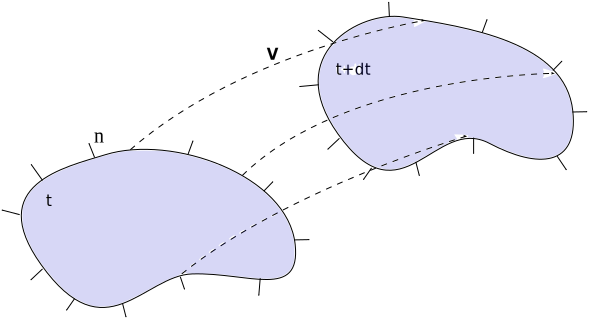
\includegraphics[width=0.7\textwidth]{principles/transportTheorem.png}
  }
  \caption{Definition of a (moving) control volume at times t and t +
    dt with contour velocity \aVelV, outward normal \nrmV.}
  \label{fig:transportTheorem}
\end{figure}
Throughout the course we will consider flow through fixed or moving
control volumes, such as shown in figure
\ref{fig:transportTheorem}. We first denote such a closed control
volume by $\vol$ and its contour by $\srf$; this control volume may
move and deform in time with a local speed $\aVelV_\vol(\xyzV,t)$. The
most commonly used integral theorems are
\begin{itemize}
\item for the gradient of a scalar:
  \begin{align*}
    \int_{\vol} \grad a ~ dV = \oint_{\srf} a~\nrmV~dS 
  \end{align*}
\item for the divergence of a vector (Gauss theorem):
  \begin{align*}
    \int_{\vol} \dive \mathbf a~dV = \oint_{\srf} \mathbf a \cdot \nrmV~dS 
  \end{align*}
\item for the divergence of a dyadic 
  \begin{align*}
    \int_{\vol} \dive \stressT~dV = \oint_{\srf} \stressT \cdot \nrmV~dS
  \end{align*}
\end{itemize}

% Using the chain rule for derivation and the above integral theorems,
% we can easily derive a number of partial integration rules. For
% instance, since $\dive a \mathbf b = a \dive \mathbf b + \mathbf b
% \cdot \grad a$, we have
% \begin{align*}
%   \int_{\vol} a \dive \mathbf b = 
%   \int_{\srf} a \mathbf \cdot \nrmV dS - \int_{\vol} \mathbf b \cdot \grad a dV
% \end{align*}

% \subsection{Reynolds transport theorem}

The \emph{Reynolds transport theorem} states that the rate of change
of the integral of any quantity f on a moving control volume is equal
to the \emph{integral of the rate of change of f on the original
  volume} and the \emph{its flux across the contour of the volume as
  it moves}:
\begin{align*}
  \begin{split}
    \ddtM{} \int_{\vol(t)} f dV = \int_{\vol} \ddt{f} dV +
    \oint_{\srf} f \aVelV_\vol \cdot \nrmV~dS
  \end{split}
\end{align*}
with $\aVelV_\vol$ the velocity of the boundary of the control volume

\subsection{Material derivative}

\begin{figure}[H]
  \centering{
    \includegraphics[width=0.7\textwidth]{principles/materialDerivative.png}}
  \caption{Computation of the material derivative}
\end{figure}

The \emph{material derivative} is the time derivative experienced by a
material particle as it moves along its path. Say that it is located
at $\xyzV(t)$ at time t. At $t+dt$ it will have moved over $d\xyzV =
\aVelV~ dt + \mathcal O(dt^2)$. The material derivative is then found
by Taylor expansion
\begin{align*}
  \frac{d a}{dt} 
  &= \lim_{dt \rightarrow 0} \frac{a(\xyzV + d\xyzV,t+dt) - a(\xyzV,t)}{dt} \\ 
  &= \lim_{dt \rightarrow 0} \frac{1}{dt} 
  \left(a(\xyzV,t) + dt~\ddt{a} + \aVelV~dt \cdot \grad a + \mathcal O(dt^2) - a(\xyzV,t)\right) \\
  &= \ddt{a} + \aVelV \cdot \grad a
\end{align*}
as the combination of the \emph{local} time derivative and the
convection term.

%%% Local Variables: 
%%% mode: latex
%%% TeX-master: t
%%% End: 
